\documentclass[journal]{IEEEtran}

\usepackage{graphicx} 
\usepackage{caption} 
\usepackage{siunitx} 
\usepackage{subcaption} 
\captionsetup[table]{skip=10pt}
\usepackage[margin=1in]{geometry} 
\usepackage{amsmath,amsthm,amssymb}
\usepackage[noend]{algpseudocode}
\usepackage{float}
\makeatletter
\def\BState{\State\hskip-\ALG@thistlm}
\makeatother

\graphicspath{{media/}}

\begin{document}

\title{Team 9 ROB 550 BotLab}

\author{Peter Mitrano, Sid Dey, Nathaniel Cox}

\maketitle

\begin{abstract}
In the BalanceBot lab, teams are tasked with autonomous and manual navigation with an two wheeled segway style vehicle. In this report, we present our approach to the BalanceBot lab. We describe the design and implementation of our motor model, controller, odometry, and planning systems. Finally, we discuss the results on the competition tasks.
\end{abstract}
\IEEEpeerreviewmaketitle

\section{Introduction}
\IEEEPARstart{T}{h}e goal of the BotLab lab is to 

\section{Methods}

\subsection{PID Gains}

1.0 0.0 0.0 25
01.00.0 0.0 25
0.05 0.0 0.0 10
0.05 0.0 0.0 10

\subsection{Motion Controller}

Describe and document your motion control algorithm for getting between waypoints if it is different from the provided motion\_controller program.

Include a plot of your robot’s dead reckoning estimated pose and the ground truth pose from the optitrack system as the robot is commanded to drive a square 4 times using the drive\_square program.

\subsection{Monte Carlo Localization}

\subsubsection{Occupancy Grid}

Include an image of your map from the log file obstacle\_slam\_10mx10m\_5cm.log

\begin{figure}
    \centering
    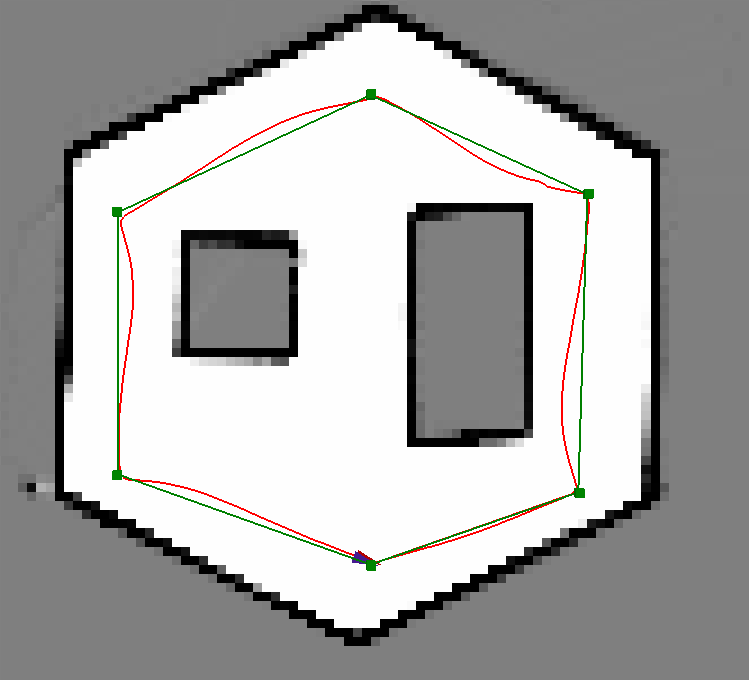
\includegraphics[width=1\linewidth]{obstacle_slam_10mx10m_5cm-map.png}
    \caption{Map built on the log file obstacle\_slam\_10mx10m\_5cm.log. True pose of the robot is shown in red.}
    \label{fig:map}
\end{figure}


\subsubsection{Action Model}

Describe the action model you used.  Include the equations you used
Include a table of the values of any uncertainty parameters.  
Explain how you chose these values.

\subsubsection{Sensor Model}

Describe the sensor model you implemented.

\subsubsection{Particle Filter}

Report in a table the time it takes to update the particle filter for 100, 300, 500 and 1000 particles.  Estimate the maximum number of particles your filter can support running at 10Hz on the RPi.
Using your particle filter on the log drive\_square\_10mx10m\_5cm.log, plot 300 particles at the midpoint of each 1m translation and at the corners after having turned 90° 

\subsection{SLAM}

Create a block diagram of how the SLAM system components interact
Compare your estimated poses against the ground-truth. Create a table showing the performance of your SLAM implementation vs. ground-truth (via motion capture). Show the mean, stdev, and max of the pose error for obstacle\_slam\_10mx10m\_5cm.log. 
Using drive\_square with 4 complete circuits, log your SLAM pose estimate in a convex environment in addition to odometry and ground truth and plot these on a completed map.
Provide a separate plot showing how the pose error evolves over time. 
\subsection{Exploration}

Provide a figure showing the planned path in an environment of your creation with the actual path driven by your robot overlayed on top. 
Using astar\_test\_files, please report statistics on your path planning execution times for each of the example problems in the data/astar folder -- you simply need to run astar\_test\_files after implementing your algorithm. If your algorithm is optimal and fast, great. If not please discuss possible reasons and strategies for improvement.

Explain the strategy used for localization in this instance and any other details about your implementation that you found important for making your algorithm work.

\section{Results}

how we picked parameters:
kzRand, we checked (kzRand/6)^32 and make sure it wasn't numeric underflow

\section{Discussion}

\section{Conclusion}

Group 9 successfully completed the BotLab lab, ...

\bibliographystyle{IEEEtran}
\bibliography{550-botlab}

\newpage

\section{Appendix}

\end{document}